% Chapter 1
\chapter{ویژگی‌های نسخه جدید \lr{Openflow}}
همانگونه که در فصل قبل گفته شد، پروتکل \lr{Openflow} همواره در حال عرضه نسخه‌های جدید می‌باشد تا بتواند پاسخگوی نیاز‌ها به روز و پویای شبکه و همچنین رفع مشکلات نسخه‌های پیشین باشد. در شکل \ref{fig7} تغییرات عمده و مهم این پروتکل در بازه زمانی عرضه آن با نسخه \lr{OF1.0} تا هم اکنون (سال ۲۰۲۱ میلادی) که نسخه \lr{OF1.5.1} به صورت استاندارد قابل دسترس است را مشاهده می‌کنیم.

\begin{figure}[H]
	\centering
	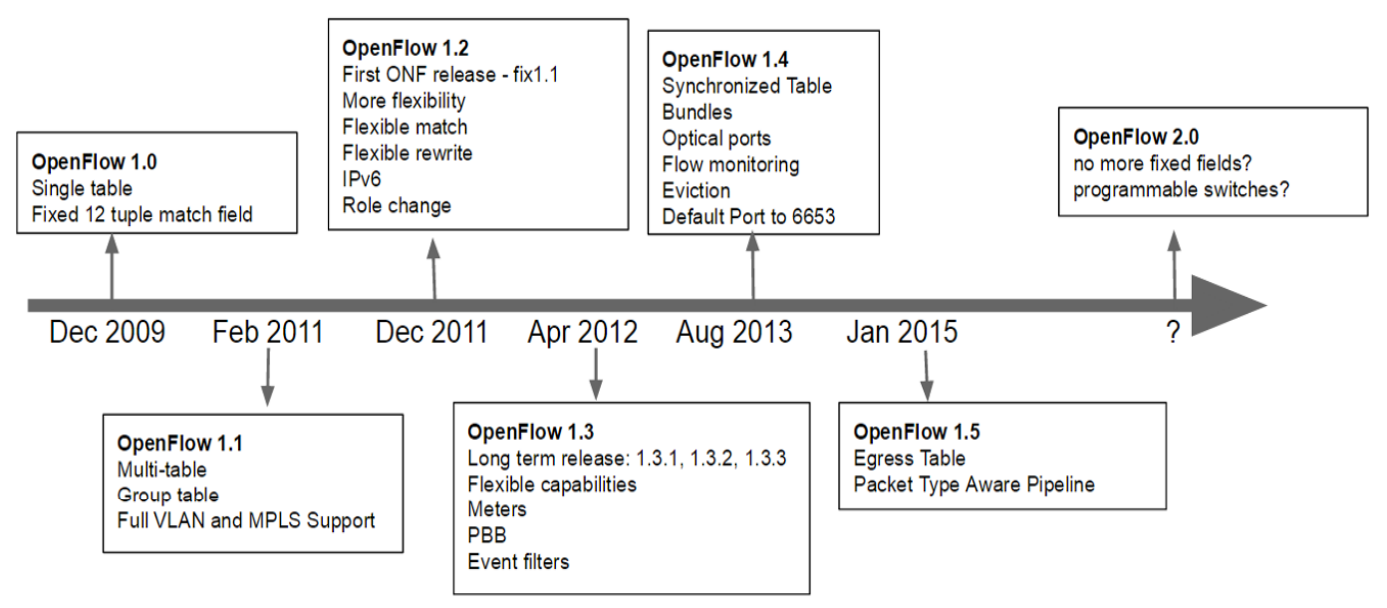
\includegraphics[scale=0.4]{imgs/of_timeline.png}
	\caption{روند پیشرفت پروتکل در نسخه‌های مختلف}
	\label{fig7}
\end{figure}

\pagebreak

\section{ویژگی‌های نسخه \lr{OF1.5}}
ویژگی‌های این نسخه را می‌توان در سه دسته، طبقه‌بندی کرد: اضافه شده‌ها، بهبود یافته‌ها و تغییرات. اضافه شده‌ها، ویژگی‌های کاملا جدیدی هستند که به پروتکل اضافه شده‌اند؛ بهبود یافته‌ها به منظور کامل کردن بخش‌های موجود در پروتکل اضافه شده اند و تغییرات نیز بخش‌هایی از پروتکل هستند که به صورت کامل دستخوش تغییر شده‌اند.
برخی از مهم‌ترین ویژگی‌های این نسخه عبارت‌اند از (تعدادی از ويژگی‌ها به دلیل جزئی بودن ذکر نشده است):

\begin{enumerate}[label=\Alph*]
	\item 
اضافه شده‌ها
	\begin{itemize}[noitemsep,topsep=0pt,parsep=0pt,partopsep=0pt]
		\item جداول جریان خروجی
		\item مهم بودن نوع بسته در خط لوله
		\item \lr{Extensible Flow Entry Statistics (OXS)}
		\item ارسال خودکار آماره‌های مدخل جریان
		\item عملیات \lr{Copy-Field}
		\item فیلد‌های خط لوله \lr{Packet Register}
		\item تطابق \lr{TCP flags}
		\item وضعیت ارتباط کنترل کننده
	\end{itemize}
	\item
بهبود یافته‌ها
	\begin{itemize}[noitemsep,topsep=0pt,parsep=0pt,partopsep=0pt]
		\item دستورات تکاملی گروه برای تغییرات انتخابی در سطل‌ها
		\item قابلیت عملیات \lr{set-field} برای تنطیم فراداده‌ها
		\item اجازه استفاده از \lr{wildcard} در عملیات \lr{set-field}
		\item \lr{Scheduled Bundles}
	\end{itemize}
	\item
تغییرات
	\begin{itemize}[noitemsep,topsep=0pt,parsep=0pt,partopsep=0pt]
		\item تغییر \lr{Meter instruction} به \lr{Meter action}
	\end{itemize}
\end{enumerate}

در ادامه گزارش به شرح هر یک از تغییرات و کاربرد‌های آن‌ها می‌پردازیم.
\pagebreak

\subsection{جداول جریان خروجی}
در نسخه‌های قبلی تمام پردازش روی بسته‌ها در حیطه‌ی درگاه ورودی انجام می‌شد. اما در نسخه \lr{OF1.5} با معرفی جداول جریان خروجی\LTRfootnote{Egress Flow Tables}، قابلیت پردازش بسته‌ها در حیطه‌ی پورت خروجی نیز فراهم می‌گردد. زمانی که بسته برای خروجی به درگاه مربوط ارجاع داده می‌شود، پردازش این بخش در اولین جدول جریان خروجی آغاز می‌شود که طی آن عملیات‌های مورد نظر روی بسته انجام شده یا به جداول دیگر خروجی ارجاع داده می‌شود. از ویژگی‌های این مرحله از پردازش می‌توان به موارد زیر اشاره کرد:
\begin{itemize}
	\item
تمام پردازش‌های مرتبط با پورت‌های منطقی، جداول جریان ورودی و جدول گروه قبل از این بخش انجام می‌شوند.
	\item
تعریف رفتار جدول جریان خروجی و مدخل‌های جریان آن بسیار شبیه به ورودی است.
	\item
قابلیت تغییر درگاه خروجی در این جداول وجود ندارد.
	\item
تمام فراداده‌های مربوط به خط لوله از پردازش  ورودی به پردازش خروجی منتقل می‌شوند.
	\item
مجموعه عملیات پردازش خروجی در ابتدا با عملیات خروجی پر شده است که در برابر مجموعه عملیات ورودی  که تهی می‌باشد متفاوت است.
\end{itemize}
استفاده از پردازش قبل از خروجی از این جهت حائز اهمیت می‌باشد که در این مرحله از پردازش، درگاه خروجی و وضعیت نهایی بسته طی مراحل قبلی مشخص شده است و می‌توان عملیات‌های این بخش را با توجه به شرایط جدید انجام داد که این خود آزادی عمل بیشتری در تطابق و ایجاد تغییر در بسته‌ها را به ارمغان می‌آورد.


